
\chapter{绪论}

\label{chap:introduction}
社会影响无处不在,不仅存在于我们的日常生活中,也存在于虚拟网络空间中。“社会 影响”一词通常指一个人的情绪、观点或行为受到他人影响的现象。随着在线和移动社交平台的全球普及,人们已经看到了社会影响在各个领域的影响,如总统选举\cite{2012political}、广告\cite{v011a004}等等。到目前为止,毫无疑问,社会影响已经成为推动我们社会决策的一种普遍而复杂的力量,明确需要方法来描述、理解和量化社会影响的基本机制和动态。


\begin{figure}[!htbp]
    \centering
    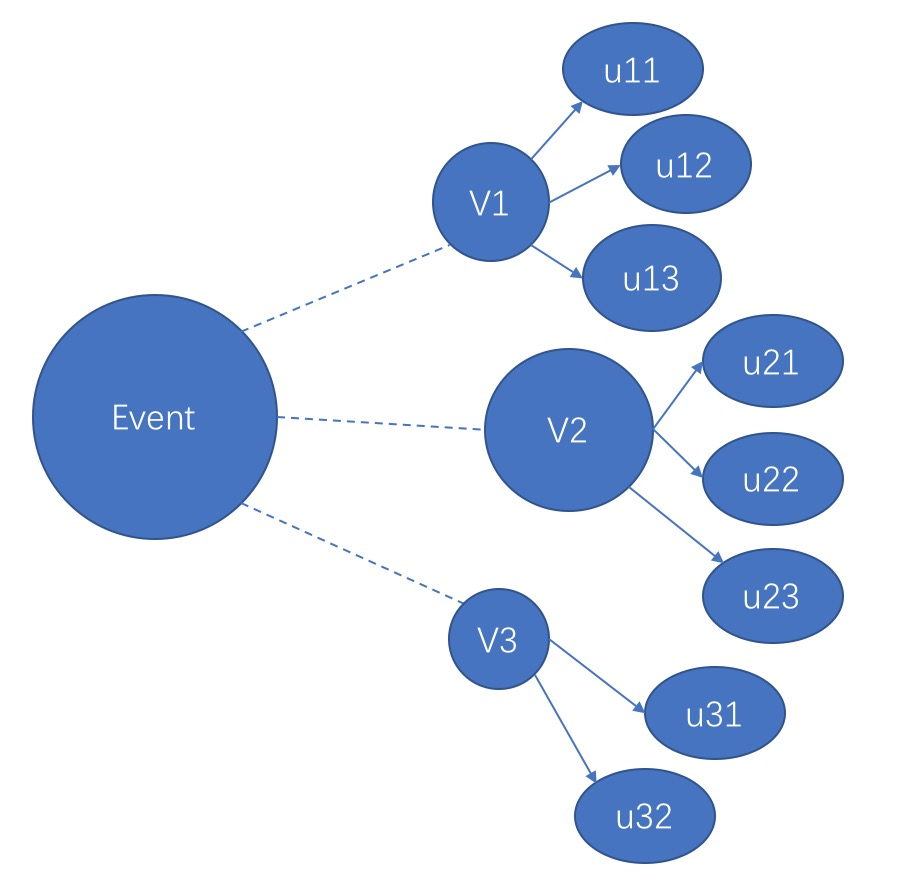
\includegraphics[width=0.50\textwidth]{Event}
    \caption{热点事件传播示意图}
    \label{fig:Event}
\end{figure}

\section{研究现状}\label{sec:status}

事实上,许多文献都对社会影响预测做了大量的工作。例如,Matsubara等人\cite{Rise2012fall}通过精心设计从经典的“易感染”模型扩展而来的微分方程,研究了社会影响的动力学。最近,Li等人\cite{DBLP:journals/corr/LiMGM16}出了一种结合递归神经网络(RNN)和表示学习来推断级联大小的端到端预测方法。所有这些方法的主要目的是预测社会影响的全球或聚集模式,如在一个时间框架内的级联规模。然而,在许多在线应用中,如广告和推荐,有效地预测每个人的社会影响是至关重要的,即用户层面的社会影响预测。像Twitter这样的西方在线社交网络已经得到了很好的研究,但中国人气颇高的微博网络新浪微博的特点却一直很少被研究过。文献\cite{2012arXiv1202.0327Y}发现,转发在新浪微博上更加普遍,并为创造趋势做出了很大贡献。

国内文献\cite{2019TSRank}\cite{2016PSO}\cite{2018UserInfluenc}\cite{2015similarity}尝试对于微博社交影响力进行多个角度的研究。其中文献\cite{2016PSO}提出将粒子群算法应用于热点话题的发现,得出结果表明用户的转发操作对话题的影响力有比较大的影响的结论。文献\cite{2019TSRank}考虑用户话题信息传播能力以及用户与背景话题间关联性,提出了TSRank算法,但是上述论文都没有考虑使用者在整个社群网络结构中的各种重要程度。



本文主要研究用户层面的社会影响预测。我们的目的是通过某一热点话题在转发过程中不同用户的行动状态,用户的近邻的动作状态和该话题被转发的的结构信息,给出该热点话题的影响力。例如,在图\ref{fig:Event}中,当热点事件发生之后,常常是社区中的意见领袖刷线发布原创内容,经过普通用户层层传递,持续活跃直至周期结束。

\begin{figure}[!htbp]
    \centering
    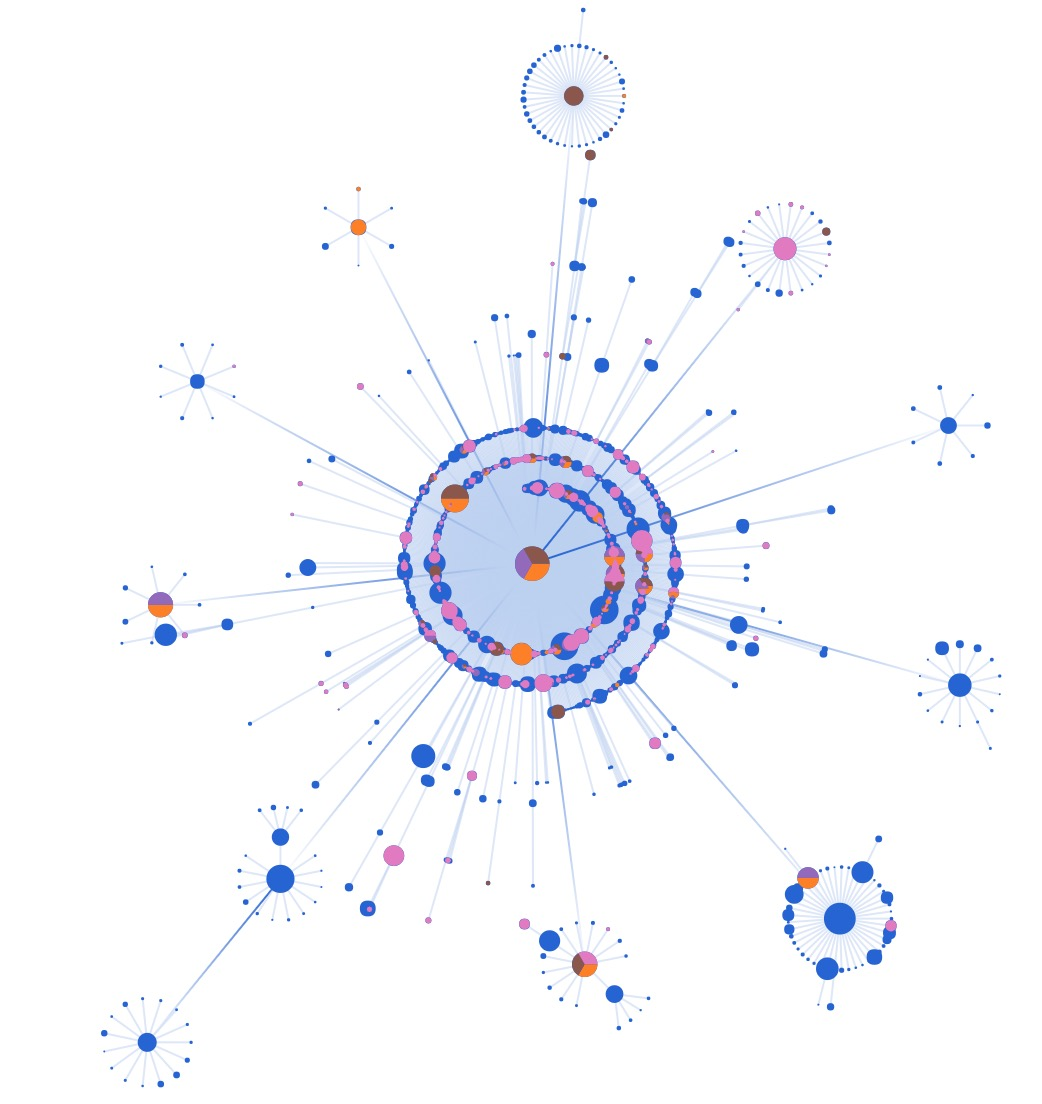
\includegraphics[ width=0.50\textwidth]{Circular}
    \caption{社交用户转发关系图(不同的颜色表示不同关键词)}
    \label{fig:Circular}
\end{figure}

受到社交相似性在微博转发中的预测成功的启发\cite{2015similarity},我改进了基于GHSOM\cite{2018UserInfluenc}算法,发现社会影响中隐藏的和预测的信号。通过将网络嵌入\cite{Qiu:2018:NEM:3159652.3159706}、图卷积\cite{kipf2017semi}和SOM神经网络构建到一个方案中。在获得如图\ref{fig:Circular}所示的转发网络后,我们利用图卷积技术来补齐关键特征。然后经过GHSOM神经网络将高维特征中隐藏的信息映射到二维网络上,结合网络特征和自定义的手工特征计算社会影响力。经过广泛的实验,结果表明,模型可以方法能准确及有效评估微博用户的影响力。

\newtheorem{theorem}{定义}[subsection]
\section{问题特征}\label{sec:question}

\subsection{顶点特征}
\begin{theorem}[度中心性]
连结度中心性为该节点与其邻居节点的所有连结数的总合。
\end{theorem}
如式(\ref{con:degreeCentrality})所示。
\begin{equation}
C_D(n_i)=degree_{in}(n_i)+degree_{out}(n_i)
\label{con:degreeCentrality}
\end{equation}
式(\ref{con:degreeCentrality})中,$degree_{in}(n_i)$ 代表其 他使用者连到$n_i$使用者的连结数,$degree_{out}(n_i)$为使用者$n_i$连到其他使用者的连结数。



\begin{theorem}[邻近度中心性]
邻近度中心性则是以该节点与其余所有在同一网络中的节点的距离总和来做计算。
\end{theorem}
\begin{equation}
C_c(n_i)=\frac{1}{\sum_{k\neq1} distance(n_i,n_j)}
\label{con:closenessCentrality}
\end{equation}
如式(\ref{con:closenessCentrality})所示。式(\ref{con:closenessCentrality})中,$distance(n_i,n_j)$为$n_i$到$n_j$节点的距离。





\begin{theorem}[中介度中心性]
中介度中心性则是用来计算除了该节点外的所有节点中,任两节点之间的路径中,通过该节点的路径数除以此两节点所有路径数比值的总合。
\end{theorem}
当节点在网络 中扮演着链接两个原先互不相连的节点之角色时,该节点中介度中心性的值则会较高,
\begin{equation}
C_B(n_i)=\sum_{j,k\neq i}\frac{|path_{via n_i}(n_i,n_k)|}{|path_{total}(n_j,n_k)|}
\label{con:betweennessCentrality}
\end{equation}
如式(\ref{con:betweennessCentrality})所示。式(\ref{con:betweennessCentrality})中,$path_{via n_i}(n_i,n_k)$为节点$n_j$通过节点$n_i$而连结到节点$n_k$的最短路径数,$path_{total}(n_j,n_k)$则为节点$n_j$连 结到节点$n_k$的所有最短路径数。





\subsection{手工特征}

Repost influence 则是用户本月所 发布的信息被转发次数的平均,该项指针能反映出使 用者所发布之言论的价值。
式(\ref{con:repostInf})中,
$N_m$为使用者每月所发布之信息量,而$\sum N_R$则为每月 每则信息被转发次数之总和。
\begin{equation}
I_r=1-\sqrt{\frac{N_m}{N_m+\sum N_R}}
\label{con:repostInf}
\end{equation}

Repost depth 转发深度,用章节\ref{sec:analyse}中的被转发的层数的最大值来评估。


Mention influence 为用户每月所发布之信息被 回复及评论的次数,该项指标反映出使用者能吸引多 少追随者来参与对话的能力,也就是言论话题性。
式(\ref{con:mentionInf})中,$N_M$为使用者每月所发布之信息
量,$\sum N_M$则为每月每则信息被讨论次数之总和。
\begin{equation}
I_m=1-\sqrt{\frac{N_m}{N_m+\sum N_M}}
\label{con:mentionInf}
\end{equation}


Geographical influence 地理影响分布,参考\href{https://open.weibo.com/wiki/%E7%9C%81%E4%BB%BD%E5%9F%8E%E5%B8%82%E7%BC%96%E7%A0%81%E8%A1%A8}{新浪微博的省份城市编码},比如,宁夏的省份编号是64,其下的主要城市分别为1银川、2石嘴山、3吴忠、4固原,青海的省份编号是63,其下主要城市有8个。我们发现地理上相邻的省份及城市,其编号也非常接近,我们建立影响广度特征公式(\ref{con:geoInf})。其中$P$表示省份,$C$表示城市,$I_{i,j}$表示在省份P下的城市C被影响的个数。
\begin{equation}
I_g=\frac{1}{P}\sum_{i\in P}\sum_{j\in C}\frac{I_{i,j}}{I_{i,total}}
\label{con:geoInf}
\end{equation}


检验预测结果的方法。
Spearman’s rank correlation coefficients是用来 分析两种排名算法之间相关性的量测方法。
如式(\ref{con:spearman})所示。该分析方法是根据等级数据研究两个变量间相关 性的方法,相关性越高其分析结果越接近+1,相关性 越低其分析结果越接近-1。

\begin{equation}
\rho=1-\sqrt{\frac{6\sum (x_i-y_i)}{N(N^2-1)}}
\label{con:spearman}
\end{equation}
